%%%%%%%%%%%%%%%%%%%%%%%%%%%%%%%%%%%%%%%%%
% Beamer Presentation
% LaTeX Template
% Version 1.0 (10/11/12)
%
% This template has been downloaded from:
% http://www.LaTeXTemplates.com
%
% License:
% CC BY-NC-SA 3.0 (http://creativecommons.org/licenses/by-nc-sa/3.0/)
%
%%%%%%%%%%%%%%%%%%%%%%%%%%%%%%%%%%%%%%%%%

%----------------------------------------------------------------------------------------
%	PACKAGES AND THEMES
%----------------------------------------------------------------------------------------

\documentclass{beamer}

\mode<presentation> {

% The Beamer class comes with a number of default slide themes
% which change the colors and layouts of slides. Below this is a list
% of all the themes, uncomment each in turn to see what they look like.

% \usetheme{default}
% \usetheme{AnnArbor}
% \usetheme{Antibes}
% \usetheme{Bergen}
% \usetheme{Berkeley}
% \usetheme{Berlin}
\usetheme{Boadilla}
% \usetheme{CambridgeUS}
% \usetheme{Copenhagen}
% \usetheme{Darmstadt}
% \usetheme{Dresden}
% \usetheme{Frankfurt}
% \usetheme{Goettingen}
% \usetheme{Hannover}
% \usetheme{Ilmenau}
% \usetheme{JuanLesPins}
% \usetheme{Luebeck}
% \usetheme{Madrid}
% \usetheme{Malmoe}
% \usetheme{Marburg}
% \usetheme{Montpellier}
% \usetheme{PaloAlto}
% \usetheme{Pittsburgh}
% \usetheme{Rochester}
% \usetheme{Singapore}
% \usetheme{Szeged}
% \usetheme{Warsaw}

% As well as themes, the Beamer class has a number of color themes
% for any slide theme. Uncomment each of these in turn to see how it
% changes the colors of your current slide theme.

%\usecolortheme{albatross}
%\usecolortheme{beaver}
%\usecolortheme{beetle}
%\usecolortheme{crane}
%\usecolortheme{dolphin}
%\usecolortheme{dove}
%\usecolortheme{fly}
%\usecolortheme{lily}
%\usecolortheme{orchid}
%\usecolortheme{rose}
%\usecolortheme{seagull}
%\usecolortheme{seahorse}
%\usecolortheme{whale}
%\usecolortheme{wolverine}

%\setbeamertemplate{footline} % To remove the footer line in all slides uncomment this line
%\setbeamertemplate{footline}[page number] % To replace the footer line in all slides with a simple slide count uncomment this line

%\setbeamertemplate{navigation symbols}{} % To remove the navigation symbols from the bottom of all slides uncomment this line
}

\usepackage{graphicx} % Allows including images
\usepackage{booktabs} % Allows the use of \toprule, \midrule and \bottomrule in tables
\usepackage{caption}

%----------------------------------------------------------------------------------------
%	TITLE PAGE
%----------------------------------------------------------------------------------------

\title[Text Generation in Discrete Space]{Text Generation in Discrete Space} % The short title appears at the bottom of every slide, the full title is only on the title page

\author[M. Zhao et F. Mi]{\underline{Mengjie Zhao}  \and Fei Mi } % Your name
\institute[] % Your institution as it will appear on the bottom of every slide, may be shorthand to save space
{
\footnotesize{Artificial Intelligence Laboratory (LIA)}
\date{\today}
\\\medskip
\medskip
\medskip
\medskip
\medskip
\medskip
% \footnotesize{\'Ecole polytechnique f\'ed\'erale de Lausanne} \\ % Your institution for the title page
\medskip
% \textit{john@smith.com} % Your email address
\vspace{-1cm}
\begin{figure}
\includegraphics[width=0.2\linewidth]{imgs/epfl1.eps}
\end{figure}
}

 % Date, can be changed to a custom date

\begin{document}
\begin{frame}
\titlepage % Print the title page as the first slide
\end{frame}

\begin{frame}
\frametitle{Some info about me...} 
\begin{itemize} 
\item Mengjie (Joe) Zhao
\item MS student from communication systems
\end{itemize}
\end{frame}

\begin{frame}
\frametitle{Overview} % Table of contents slide, comment this block out to remove it
\tableofcontents % Throughout your presentation, if you choose to use \section{} and \subsection{} commands, these will automatically be printed on this slide as an overview of your presentation
\end{frame}

%----------------------------------------------------------------------------------------
%	PRESENTATION SLIDES
%----------------------------------------------------------------------------------------

%------------------------------------------------
\section{Generative Adversarial Networks (GANs)} % Sections can be created in order to organize your presentation into discrete blocks, all sections and subsections are automatically printed in the table of contents as an overview of the talk
%------------------------------------------------

\begin{frame}
\frametitle{The generative model}
\begin{figure}
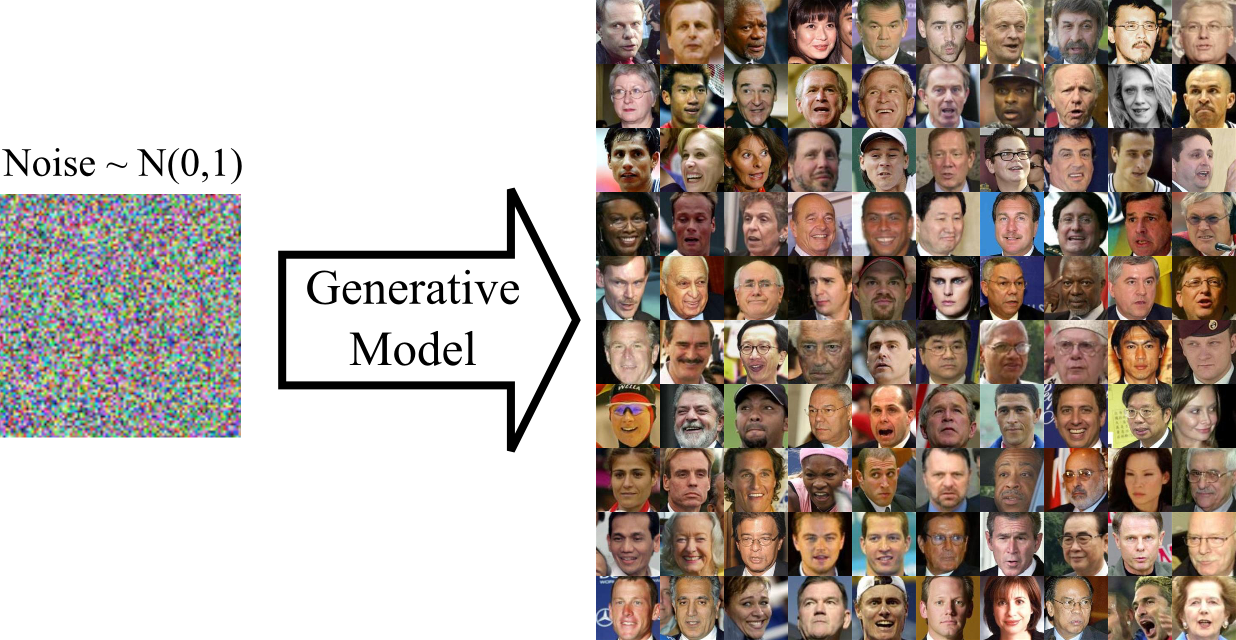
\includegraphics[width=0.8\linewidth]{imgs/w1_g_model.png}
\end{figure}
\hspace{7cm}\tiny{src: http://torch.ch/blog/2015/11/13/gan.html}
\end{frame}


%------------------------------------------------

%------------------------------------------------

\begin{frame}
\frametitle{Generative Adversarial Networks (GANs)}
\begin{figure}
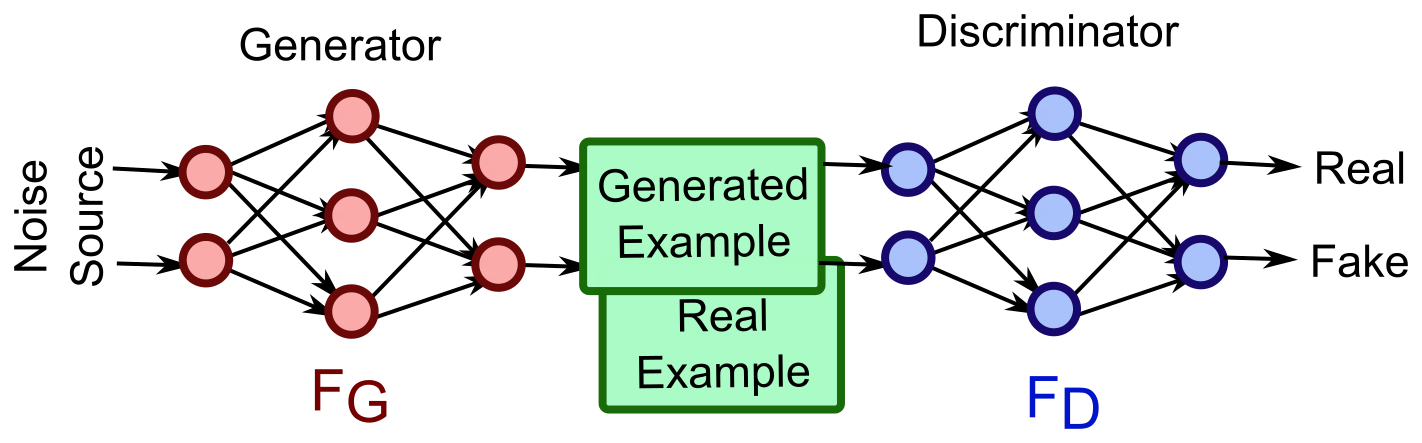
\includegraphics[width=0.8\linewidth]{imgs/w1_gan.png}
\end{figure}
\vspace{1cm}
\hspace{7cm}\tiny{src: http://www.araya.org/archives/1183}
\end{frame}

%------------------------------------------------

%------------------------------------------------

\begin{frame}
\frametitle{To be more formal}
\begin{itemize}
\item Define $p_{data}$ as the distribution where data generated from
\item Input noise $\textbf{z}$ from noise distribution $p_z(z)$
\item Generator: $G(z;\theta_{g}) \Rightarrow \textbf{x}$
\item Discriminator: $D(\textbf{x}; \theta_{d})$
\item Two-player minimax game with value function $V(G, D)$:
\end{itemize}
\begin{figure}
\includegraphics[width=0.8\linewidth]{imgs/game}
\end{figure}
\end{frame}

%------------------------------------------------

%------------------------------------------------

\begin{frame}
\frametitle{To be more cartoon...}
\begin{figure}
\includegraphics[width=\linewidth]{imgs/gan_numeric}
\end{figure}
\vspace{1cm}
\hspace{9cm}\tiny{(Goodfellow et al. 2014)}
\end{frame}
%------------------------------------------------

%------------------------------------------------
\begin{frame}
\frametitle{Performance of a toy GAN (full connected MLPs)}
\begin{figure}
\centering
\begin{minipage}{.5\textwidth}
  \centering
  \includegraphics[width=.62\linewidth]{imgs/gan_generated_img_e_50.png}
  \captionof{figure}*{Generated letters from G (50 epochs)}
  \label{fig:test1}
\end{minipage}%
\begin{minipage}{.5\textwidth}
  \centering
  \includegraphics[width=.83\linewidth]{imgs/loss_d.eps}
  \captionof{figure}*{Loss of D (50 epochs)}
  \label{fig:test2}
\end{minipage}
\end{figure}
\end{frame}
%------------------------------------------------



% \begin{frame}
% \frametitle{Bullet Points}
% \begin{itemize}
% \item Lorem ipsum dolor sit amet, consectetur adipiscing elit
% \item Aliquam blandit faucibus nisi, sit amet dapibus enim tempus eu
% \item Nulla commodo, erat quis gravida posuere, elit lacus lobortis est, quis porttitor odio mauris at libero
% \item Nam cursus est eget velit posuere pellentesque
% \item Vestibulum faucibus velit a augue condimentum quis convallis nulla gravida
% \end{itemize}
% \end{frame}

%------------------------------------------------

% \begin{frame}
% \frametitle{Blocks of Highlighted Text}
% \begin{block}{Block 1}
% Lorem ipsum dolor sit amet, consectetur adipiscing elit. Integer lectus nisl, ultricies in feugiat rutrum, porttitor sit amet augue. Aliquam ut tortor mauris. Sed volutpat ante purus, quis accumsan dolor.
% \end{block}

% \begin{block}{Block 2}
% Pellentesque sed tellus purus. Class aptent taciti sociosqu ad litora torquent per conubia nostra, per inceptos himenaeos. Vestibulum quis magna at risus dictum tempor eu vitae velit.
% \end{block}

% \begin{block}{Block 3}
% Suspendisse tincidunt sagittis gravida. Curabitur condimentum, enim sed venenatis rutrum, ipsum neque consectetur orci, sed blandit justo nisi ac lacus.
% \end{block}
% \end{frame}

%------------------------------------------------

% \begin{frame}
% \frametitle{Multiple Columns}
% \begin{columns}[c] % The "c" option specifies centered vertical alignment while the "t" option is used for top vertical alignment

% \column{.45\textwidth} % Left column and width
% \textbf{Heading}
% \begin{enumerate}
% \item Statement
% \item Explanation
% \item Example
% \end{enumerate}

% \column{.5\textwidth} % Right column and width
% Lorem ipsum dolor sit amet, consectetur adipiscing elit. Integer lectus nisl, ultricies in feugiat rutrum, porttitor sit amet augue. Aliquam ut tortor mauris. Sed volutpat ante purus, quis accumsan dolor.

% \end{columns}
% \end{frame}
\begin{frame}
\frametitle{Overview} % Table of contents slide, comment this block out to remove it
\tableofcontents % Throughout your presentation, if you choose to use \section{} and \subsection{} commands, these will automatically be printed on this slide as an overview of your presentation
\end{frame}

%------------------------------------------------
\section{Generating in discrete space?}
%------------------------------------------------

\begin{frame}
\frametitle{Generating in discrete space?}
\begin{itemize}
\item Generator and discriminator have to be differentiable.
\item But for text generation?
	\begin{itemize}
		\item word embedding
		\item policy iteration
		\item categorical reparameterisation (gumbel-softmax) ...
		% a cntinuous distribution that can approximate
		% categorical samples

	\end{itemize}
\end{itemize}
\end{frame}

%------------------------------------------------

%------------------------------------------------

\begin{frame}
\frametitle{Sequence GAN (SeqGAN) for text generation}
\begin{itemize}
\item Treat generator as an agent in reinforcement learning
	\begin{itemize}
		\item State: generated tokens so far
		\item Action: next token to be generated
		\item Reward: evaluation of the sequence from D
		\item \textbf{Policy iteration}
	\end{itemize} 
\item Experimental performance:
\begin{figure}
\centering
\includegraphics[width=0.75\linewidth]{imgs/pre_cru}
\end{figure}
\vspace{-.2cm}
\hspace{9cm}\tiny{(Yu et al. 2017)}
\end{itemize}
\end{frame}

%------------------------------------------------

\begin{frame}
\frametitle{Generated sentences by SeqGAN}
\begin{itemize}
\item The Big Bang Theory subtitle dataset -- courtesy from @sudongqi
\item Some generated sentences:
	\begin{itemize}
		\item word embedding
		\item policy iteration
		\item categorical reparameterisation (gumbel-softmax) ...
		% a cntinuous distribution that can approximate
		% categorical samples

	\end{itemize}
\end{itemize}
\end{frame}

%------------------------------------------------

%------------------------------------------------
\begin{frame}
\frametitle{Dialog generation}
\begin{itemize}
\item The Big Bang Theory subtitle dataset -- courtesy from @sudongqi
\item Some generated sentences:
	\begin{itemize}
		\item word embedding
		\item policy iteration
		\item categorical reparameterisation (gumbel-softmax) ...
		% a cntinuous distribution that can approximate
		% categorical samples

	\end{itemize}
\end{itemize}
\end{frame}

%------------------------------------------------

% \begin{frame}
% \frametitle{Theorem}
% \begin{theorem}[Mass--energy equivalence]
% $E = mc^2$
% \end{theorem}
% \end{frame}

%------------------------------------------------

% \begin{frame}[fragile] % Need to use the fragile option when verbatim is used in the slide
% \frametitle{Verbatim}
% \begin{example}[Theorem Slide Code]
% \begin{verbatim}
% \begin{frame}
% \frametitle{Theorem}
% \begin{theorem}[Mass--energy equivalence]
% $E = mc^2$
% \end{theorem}
% \end{frame}\end{verbatim}
% \end{example}
% \end{frame}

%------------------------------------------------

% \begin{frame}
% \frametitle{Figure}
% Uncomment the code on this slide to include your own image from the same directory as the template .TeX file.
% %\begin{figure}
% %\includegraphics[width=0.8\linewidth]{test}
% %\end{figure}
% \end{frame}

%------------------------------------------------
\section{Rate of progress}
%------------------------------------------------
\begin{frame}
\frametitle{Rate of progress}
\begin{figure}
\centering
\includegraphics[width=\linewidth]{imgs/gantt}
\end{figure}
\end{frame}

%------------------------------------------------
\begin{frame}
\frametitle{Overview} % Table of contents slide, comment this block out to remove it
\tableofcontents % Throughout your presentation, if you choose to use \section{} and \subsection{} commands, these will automatically be printed on this slide as an overview of your presentation
\end{frame}
%------------------------------------------------
\section{Conclusion}
%------------------------------------------------
\begin{frame}
\frametitle{Conclusion}
\begin{figure}
\centering
\includegraphics[width=\linewidth]{imgs/gantt}
\end{figure}
\end{frame}

%------------------------------------------------

% \begin{frame}[fragile] % Need to use the fragile option when verbatim is used in the slide
% \frametitle{Citation}
% An example of the \verb|\cite| command to cite within the presentation:\\~

% This statement requires citation \cite{p1}.
% \end{frame}

%------------------------------------------------
%------------------------------------------------


\begin{frame}
\vspace{3cm}
\Huge{\centerline{That's it!}}
\begin{figure}
\hspace{-7cm}
\includegraphics[width=0.2\linewidth]{imgs/bt}
\end{figure}
\end{frame}

%---------------------------------------------------

\begin{frame}
\frametitle{References}
\footnotesize{
\begin{thebibliography}{99} % Beamer does not support BibTeX so references must be inserted manually as below
\bibitem[Goodfellow et al]{p1} Goodfellow et. al. (2014)
\newblock Generative Adversarial Networks
\newblock \emph{NIPS 2014}

\bibitem[Yu et al]{p1} Yu et. al. (2017)
\newblock SeqGAN: Sequence Generative Adversarial Nets with Policy Gradient 
\newblock \emph{AAAI 17}

\bibitem[Li et. al.]{p1} Li et. al. (2017)
\newblock Adversarial Learning for Neural Dialogue Generation
\newblock \emph{arXiv:1701.06547}

\bibitem[Jang et. al.]{p1} Jang et. al. (2016)
\newblock Categorical Reparameterization with Gumbel-Softmax
\newblock \emph{arXiv:1611.01144}


\end{thebibliography}
}
\end{frame}

%-------------------------------------

\end{document}